% Exercise Template
% A LaTeX template for typesetting exercise in Persian (with cover page).
% By: Reza Adinepour
% Github: github.com/rezaAdinepour

\documentclass[12pt]{exam}

\usepackage{setspace}
\usepackage{listings}
\usepackage{graphicx,wrapfig}
\usepackage{caption}
\usepackage{subcaption}
\usepackage{multirow}
\usepackage{matlab-prettifier}
\usepackage{amsmath}
\usepackage{multicol}
\usepackage[hidelinks]{hyperref}



\usepackage[utf8]{inputenc}
\usepackage{fourier} 
\usepackage{array}
\usepackage{makecell}

\renewcommand\theadalign{bc}
\renewcommand\theadfont{\normalsize}
\renewcommand\theadgape{\Gape[4pt]}
\renewcommand\cellgape{\Gape[4pt]}


\usepackage[margin=25mm]{geometry}
\usepackage{xepersian}
\settextfont{XB Niloofar}

\newcommand{\class}{\ThesisClass}

\singlespacing
\parindent 0ex

\begin{document}


% -------------------------------------------------------
%  Thesis Information
% -------------------------------------------------------

\newcommand{\ThesisType}
{سمینار}  % پایان‌نامه / رساله
\newcommand{\ThesisDegree}
{کارشناسی ارشد گرایش معماری کامپیوتر}  % کارشناسی / کارشناسی ارشد / دکتری
\newcommand{\ThesisMajor}
{مهندسی کامپیوتر}  % مهندسی کامپیوتر
\newcommand{\ThesisTitle}
{تمرین شبیه‌سازی سری ۳}
\newcommand{\ThesisAuthor}
{\href{https://github.com/rezaAdinepour/M.Sc-AUT/tree/main/Advanced Computer Architecture}{\textcolor{black}{رضا آدینه پور}} - ۴۰۲۱۳۱۰۵۵}
\newcommand{\ThesisSupervisor}
{جناب آقای دکتر فربه}
\newcommand{\ThesisDate}
{۲۳ آذر ۱۴۰۲}
\newcommand{\ThesisDepartment}
{دانشکده مهندسی کامپیوتر}
%\newcommand{\ThesisUniversity}
%{دانشگاه صنعتی امیرکبیر}

% -------------------------------------------------------
%  English Information
% -------------------------------------------------------

%\newcommand{\EnglishThesisTitle}{A Standard Template for Course Exercise}


\pagestyle{empty}

\begin{center}


\includegraphics[scale=0.15]{images/aut-fa.png}

%\vspace{0.5cm}
%\ThesisUniversity \\[-0.3em]
%\vspace{0.5cm}
\large\ThesisDepartment

\begin{large}
\vspace{0.5cm}


%\ThesisMajor

\end{large}

\vspace{1.5cm}

{عنوان:}\\[1.2em]
{\LARGE\textbf{\ThesisTitle}}\\ 
\vspace{1cm}
% \begin{latin}
% {\Large\textbf\EnglishThesisTitle}
% \end{latin}

\vspace{2cm}

{نگارش}\\[.5em]
{\large\textbf{\ThesisAuthor}}

\vspace{1.5cm}

{استاد مربوطه}\\[.5em]
{\large\textbf{\ThesisSupervisor}}

\vspace{1cm}



\vspace{2cm}

\ThesisDate

\end{center}

\newpage


% These commands set up the running header on the top of the exam pages
\pagestyle{head}
\firstpageheader{}{}{}
\runningheader{صفحه \thepage\ از \numpages}{}{\class}
\runningheadrule

\vspace{0pt}


\begin{questions}
	\pointpoints{نمره}{نمره}
	
	
	\question
\textbf{به سوالات زیر پاسخ دهید:‌ }

\begin{enumerate}
	\item 
	\lr{PUM} چیست و کدام نوع حافظه‌ها برای آن بیشتر استفاده می‌شوند؟ توضیح دهید چرا هر نوع حافظه استفاده می‌شود.
	
	\textbf{پاسخ: }
پردازش در حافظه (\lr{PUM}) یک کانسپت محاسباتی است که در آن برخی از محاسبات ساده مانند جمع و ضرب به جای انتقال داده‌ها بین \lr{CPU} و حافظه، مستقیما در حافظه انجام می‌شوند.

معمولا از \lr{DRAM}، \lr{SRAM} و \lr{NVM} ها در \lr{PUM} استفاده می‌شود. که در ادامه به بررسی مزایا و معایب استفاده از هرکدام می‌پردازیم.

\lr{DRAM} ها
به دلیل اینکه رایج‌ترین نوع حافظه فرار با تراکم بالا و هزینه کم به ازای هر بیت هستند، به طور گسترده استفاده می‌شود. ویژگی‌های خازنی سلول‌های \lr{DRAM} امکان انجام تکنیک‌های محاسباتی درون حافظه مانند عملیات منطقی و حسابی را فراهم می‌کند.

مزایا: تراکم بالا، ارزان است.\\
معایب: فرار، نیاز به تازه‌سازی دوره‌ای و معمولاً تأخیر بیشتر نسبت به \lr{SRAM}.

اما در مقابل  \lr{SRAM} زمان‌های تأخیر کمتری و زمان دسترسی سریعتری نسبت به \lr{DRAM} دارد و در مواردی که سرعت برای ما بسیار مهم است، (مانند \lr{Cache})، استفاده می‌شود. توانایی حفظ حالت بدون نیاز به تازه‌سازی، آن را برای عملیات‌های \lr{PUM} مناسب می‌سازد.

مزایا: زمان‌های دسترسی سریع نسبت به \lr{DRAM}، عدم نیاز به تازه‌سازی.\\
معایب: تراکم کمتر و هزینه بیشتر به ازای هر بیت نسبت به \lr{DRAM}.


درمقابل حافظه‌های فرار، انواع حافظه‌های غیر فرار مانند \lr{Flash}، \lr{PCM} و \lr{ReRAM} به دلیل نگه داشتن داده بدون برق، برای ذخیره‌سازی پایدار و محاسبات مناسب هستند. این حافظه‌ها می‌توانند برخی عملیات منطقی را درون سلول‌های حافظه انجام دهند.

مزایا: غیر فرار بودن. \\
معایب: عموماً سرعت نوشتن کندتر و دوام کمتر نسبت به \lr{DRAM} و \lr{SRAM}.
	
	
	
	
	
	\item 
	نقاط ضعف \lr{UPMEM} چیست؟
	\textbf{پاسخ:} از نقاط ضعف \lr{UPMEM} ها می‌توان به موارد زیر اشاره کرد:
	
	
	\begin{enumerate}
		\item انعطاف‌پذیری و قابلیت برنامه‌ریزی محدود:\\
		
	\end{enumerate}
	. 
	
	معماری PIM UPMEM برای انواع خاصی از عملیات (مانند وظایف داده‌محور مانند جستجوهای پایگاه داده و تحلیل) تخصصی است. ممکن است به اندازه CPU یا GPUهای سنتی عمومی و همه‌منظوره نباشد، که کاربرد آن را به بارهای کاری خاص محدود می‌کند.
	
	۲. یکپارچه‌سازی و سازگاری:
	
	یکپارچه‌سازی ماژول‌های PIM UPMEM با سیستم‌های موجود می‌تواند چالش‌برانگیز باشد. ممکن است مشکلات سازگاری با معماری‌های حافظه و پردازنده فعلی به وجود بیاید که نیاز به اصلاحات در پشته نرم‌افزار و سخت‌افزار دارد.
	
	۳. مسائل مربوط به کارایی انرژی:
	
	در حالی که PIM هدفش کاهش مصرف انرژی با حداقل‌کردن حرکت داده‌هاست، صرفه‌جویی واقعی در انرژی می‌تواند وابسته به بار کاری باشد. برخی عملیات ممکن است همچنان مصرف انرژی قابل توجهی داشته باشند، به خصوص اگر منطق PIM به‌طور کامل برای وظیفه بهینه‌سازی نشده باشد.
	
	۴. مقیاس‌پذیری:
	
	مقیاس‌پذیری راه‌حل‌های PIM مانند UPMEM شامل چالش‌هایی در توازن تعداد واحدهای حافظه مجهز به PIM با معماری کلی سیستم است. مدیریت و استفاده کارآمد از تعداد زیادی واحد PIM بدون ایجاد گلوگاه‌ها یک وظیفه پیچیده است.
	
	۵. توسعه و اشکال‌زدایی:
	
	توسعه برنامه‌ها برای PIM نیاز به مدل‌های برنامه‌نویسی و ابزارهای جدید دارد. اشکال‌زدایی و پروفایل‌کردن برنامه‌های PIM می‌تواند به دلیل طبیعت توزیع‌شده و درون حافظه‌ای محاسبات سخت‌تر از برنامه‌نویسی CPU/GPU سنتی باشد.
	
	
	
	
	
	\item 
	ساختار \lr{Ambit} را معرفی کرده و مزایا و معایب آن را توضیح دهید.
\end{enumerate}

%\begin{figure}[h]
%	\centering
%	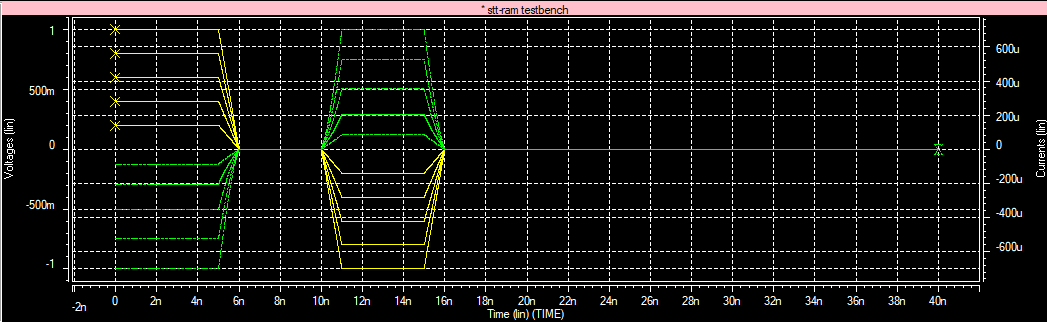
\includegraphics[width=1\textwidth]{images/img8}
%	\caption{خروجی شبیه‌سازی}
%	\label{خروجی شبیه‌سازی}
%\end{figure}

		
		
		
		
		
	
 \end{questions}

\end{document}